\section{Model matematyczny stanowiska MagLev}

Lewitacja magnetyczna to zjawisko występujące, kiedy ferromagnetyczny obiekt znajdzie się w polu magnetycznym skierowanym pionowo w górę, na tyle silnym, że wytworzona siła zrównoważy działającą na przedmiot grawitację. Zjawisko to stosuje się obecnie w łożyskach magnetycznych w pociągach, rozwijanych głównie w Japonii (MLX01) i w Niemczech (TR-08).

W laboratorium Katedry Automatyki EAIiIB AGH znajduje się stanowisko przeznaczone do badania magnetycznej lewitacji. Obiektem unoszącym się jest metalowa sfera. Pole magnetyczne jest wytwarzane przez cewkę umieszczoną ponad sferą. Dzięki pracom \cite{Bania1999}, \cite{Bania2000} i \cite{Pilat} wiemy w jaki sposób modelować zachowanie układu, a także identyfikować jego parametry fizyczne.

\begin{figure}[!htb]
\centering
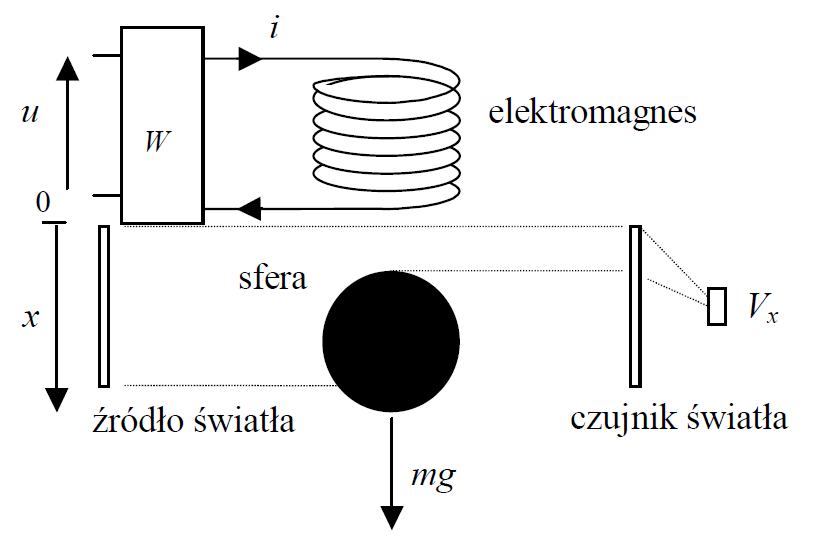
\includegraphics[scale=0.45]{img/model-rownania.PNG}
\caption{Schemat stanowiska służący do wyznaczania równań, źródło \cite{Bania2000}}
\label{rys:model-rownania}
\end{figure}

\begin{equation}\label{modelMagLev}
  \begin{cases}
    \dot x_1 & = x_2 \\
    \dot x_2 & = \dfrac{1}{2m} \dfrac{dL(x_1)}{dx_1} x_3^2(t) + 10^{-3} g  \\
    \dot x_3 & = -\frac{1}{T} x_3(t) + \frac{k}{T} (u(t) + u_c) \\
  \end{cases}  
\end{equation}

Gdzie:
\\$x_{1}$ - położenie sfery $[m]$
\\$x_{2}$ - prędkość sfery $[m/s]$
\\$x_{3}$ - prąd w cewce $[A]$ \newline

\subsection{Analiza modelu}

Zmienne stanu i sterowanie spełniają warunki:
\begin{equation}
\begin{cases}
x_1(t) \in [0, x_{max}] \\
x_2(t) \in R \\
x_3(t) \in [ku_c, k(u_c+u_{max})] \\
u(t) \in [0, u_{max}]
\end{cases}
\end{equation}



